\documentclass[twoside, 10pt]{article}

\usepackage{geometry}
\geometry{margin=2em, inner=2.5cm, top =6em, headheight=\paperheight}
\usepackage[export]{adjustbox}
\usepackage{array}
\usepackage{amsmath}
\usepackage{amsfonts}
\usepackage{fancyhdr}
\pagestyle{fancy}
\fancyhf{}
\lhead{Algebra II - BASE}
\chead{Function  Characteristics - End behaviors}
\rhead{Practice, Page \thepage}
\usepackage{lastpage}
\usepackage{xcolor}
\usepackage{enumitem}
\usepackage{pifont}
\usepackage{graphicx}
\graphicspath{{../img}}
\usepackage{pgfplots}
\pgfplotsset{compat=1.18}
\usepackage{tabularx}
\usepackage{tikz}
\usetikzlibrary{patterns}

\newcommand{\R}{\mathbb R}
\newcommand{\e}{{\rm e}}
\newcommand{\pobr}[1]{\left\langle#1\right\rangle}
\newcommand{\norm}[1]{\lVert #1 \rVert}
\newcommand{\abs}[1]{\lvert #1 \rvert}

\DeclareMathOperator{\xd}{d\!}
\DeclareMathOperator{\proj}{proj}

\title{}
\date{}

\begin{document}
\noindent
{\large
First Name \rule{6em}{.1pt}\hspace{\stretch{1}}Last Name \rule{6em}{.1pt}\hspace{\stretch{1}} Date \rule{1.5em}{.1pt} -- \rule{1.5em}{.1pt} -- \rule{1.5em}{.1pt}\hspace{\stretch{1}} Period \rule{2em}{.1pt}\hspace{\stretch{1}} Score \rule{2em}{.1pt}
}
\vspace{1em}

{\noindent \bf Learning Objectives.}
\begin{itemize}
\item
To categorize the end behaviors of the graph as approaching an infinity or a horizontal asymptote
\item
To distinguish the different pace toward infinity
\end{itemize}

{\noindent\bf Discussion.}

\begin{enumerate}[leftmargin=*]
\item
The following graph shows the state of an object cooling over time:
\begin{figure}[h]
\includegraphics[width=0.45\textwidth]{cooling-law.jpg}
\end{figure}
\begin{enumerate}
\item
What is the quantity represented by the $x$-axis?
\vspace{\stretch{1}}
\item 
What is the quantity represented by the $y$-axis?
\vspace{\stretch{1}}
\item 
How do you describe the behaviors of the graph as $x$ approaches positive infinity?
\vspace{\stretch{1}}
\item
What can you infer about the room temperature in which this cooling process was taking place? And why?
\vspace{\stretch{1}}
\end{enumerate}
\item
Suppose person $A$ has a $\$1,000,000$ annual income job, and person $B$ has a bank account with $1\%$ annual interest rate and she deposits $\$10$ in the account at the beginning. Based on these hypotheses only and ignoring any unpredictable factor. Do not turn to the flip side of this page.
\begin{enumerate}
\item
According to your intuition, who do you think is wealthier in the long run? And why?
\vspace{\stretch{1}}
\item Now turn to the flip side of the page and examine the graph. Does the graph speak to your intuition? What can you conclude now?
\clearpage
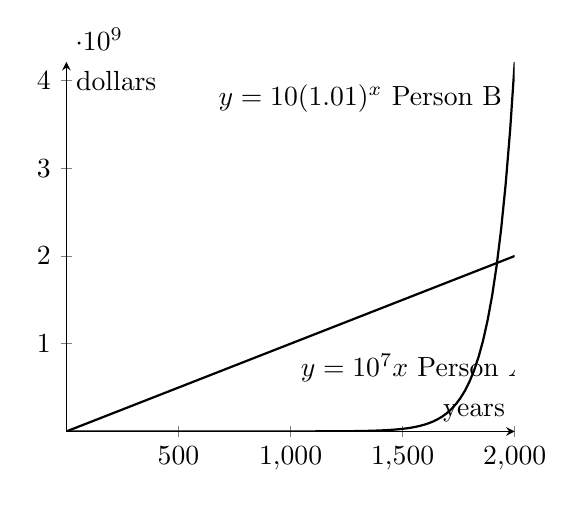
\begin{tikzpicture}
\begin{axis}[
xlabel={years},
ylabel={dollars},
axis lines=middle,
domain=0:2000,
samples=100,
width=0.6\textwidth,
]
\addplot[thick]{1000000*x}
	    node[pos=0.5, below right, black] {$y = 10^7x$ Person $A$};
\addplot[thick]{10*(1.01)^x}
		node[pos=0.9, left, black]{$y = 10(1.01)^x$ Person B};
\end{axis}
\end{tikzpicture}

(Remark: If you are unfamiliar with the concept of ``compound interest'', be sure to Google it after class!)
\vspace{\stretch{1}}
\item What life lesson can you learn from this phenomenon?
\vspace{\stretch{1}}

\end{enumerate}
\end{enumerate}

{\noindent\bf Exit Tickets.} Describe the end behaviors of the graphs below.
\begin{center}
\begin{tabular}{cc}
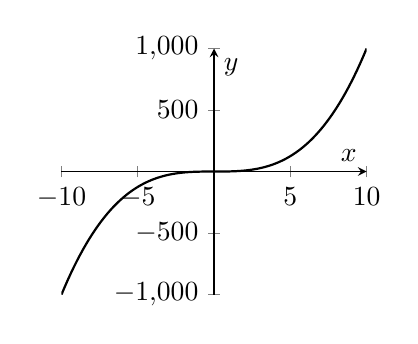
\begin{tikzpicture}
\begin{axis}[
xlabel={$x$},
ylabel={$y$},
axis lines=middle,
domain=-10:10,
samples=100,
width=0.45\textwidth,
]
\addplot[thick]{x^3};
\end{axis}
\end{tikzpicture}
&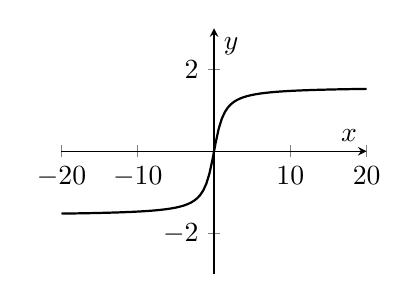
\begin{tikzpicture}
\begin{axis}[
xlabel={$x$},
ylabel={$y$},
axis lines=middle,
ymin = -3, ymax=3,
domain = -20:20,
samples=100,
width=0.45\textwidth,
]
\addplot[thick]{rad(atan(x))};
\end{axis}
\end{tikzpicture}
\end{tabular}
\end{center}
Model Statement: As $x$ approaches $\infty/-\infty$, $y$ approaches \rule{10em}{.1pt}.
\vspace{\stretch{1}}
\end{document}